% ch01 译文：原文 §1b 多重单值性、§1c Hirzebruch 面、§1d 全文结构、致谢与 AI 声明（main.tex 第 215--364 行）
\subsection{多重单值性}

除主定理中的镜像对称陈述之外，我们还能几乎不费力地得到若干重要的进一步推论。

给定 $Y$ 上的两个特征类 $\xi_1,\xi_2$，它们在辛侧的镜像辛同胚为 $\phi_1,\phi_2\in\Symp (X)$。沿零截面与无穷远截面粘合射影丛 $P(Y,\xi_i)$，即得粘合空间
\[
    \mathcal{Y} (\xi_1, \xi_2)\coloneqq P(Y,\xi_1)\cup_Y P(Y,\xi_2)
\]
% [原文 p.6]
由构造，$\mathcal{Y} (\xi_1,\xi_2)$ 仍是 $Y$ 上的纤维丛，其纤维是节点曲线 $\mathbb{P}^1\cup\mathbb{P}^1$；又因为每个 $P(Y,\xi_i)$ 都是 $\mathcal{Y}$ 的不可约分支，我们便得到真下降图表
\[
\begin{tikzcd}
    \Coh (Y)_{\infty}\arrow[r,"i_{\infty}"]\arrow[d,"i_0"]& \Coh\left(P(Y,\xi_2)\right)_{\infty}\arrow[d]\\ 
    \Coh\left(P(Y,\xi_1)\right)_{\infty}\arrow[r]&\Coh\left(\mathcal{Y} (\xi_1,\xi_2)\right)_{\infty}
\end{tikzcd}
\]
于是 $\Coh (\mathcal{Y} (\xi_1, \xi_2))_{\infty}$ 完全由该同伦前推图表决定。

\begin{yizhu}[下标 $\infty$ 与真下降的意思]
$\Coh(\,\cdot\,)_{\infty}$ 指该范畴的 $\infty$-范畴（稳定 $\infty$-范畴）版本，与带下标 $dg$ 的 dg 版本不同；文中后面借助 \cite{Cohn16} 的「dg 范畴—$\infty$-范畴」等价在两者之间来回切换。此外，这个方框图的每个顶点都是一个范畴，箭头 $i_0$、$i_\infty$ 是沿零截面、无穷远截面的包含映射所给的前推；方框图成为同伦前推图表，正是「把两个分支上的凝聚复形沿公共截面拼起来」的范畴表述，也就是「真下降」在此处的具体含义。
\end{yizhu}

与此前推图表互为镜像的是同伦前推图表
\[
    \begin{tikzcd}
        \mathcal{W} (X)\arrow[r,"\cup_0"]\arrow[d,"\cup_{\infty}"]&\mathcal{W} (M(X,\phi_2),z_2+z_2^{-1})\arrow[d]\\ 
        \mathcal{W} (M(X,\phi_1),z_1+z_1^{-1})\arrow[r]&\mathcal{W} (\mathcal{X} (\phi_1,\phi_2))
    \end{tikzcd}
\]
其中 $\mathcal{X} (\phi_1,\phi_2)$ 是把 $\left(M(X,\phi_1),z_1+z_1^{-1}\right)$ 与 $\left(M(X,\phi_2),z_2+z_2^{-1}\right)$ 沿无穷远纤维的等同 $\{z_1=\infty\}\cong\{z_2=0\}$ 粘合所得的 Weinstein 扇形。所得的扇形在去掉停止位之后，可以光滑地纤维化到带两个穿孔的圆盘 $\mathbb{D}^2\setminus\{\pm 1/2\}$ 上，停止位位于其中一个穿孔与无穷远点处。图 \ref{fig:gluing-A-model-bundle} 显示两个映射柱如何经由底空间上的粘合而拼在一起。一般地，我们可以证明下述镜像对称陈述。

\begin{yizhu}[$0$ 与 $\infty$ 的记号错位]
粘合约定很容易记反：$P(Y,\xi_1)$ 贡献的是无穷远截面，$P(Y,\xi_2)$ 贡献的是零截面，故 A 侧的等同写作 $\{z_1=\infty\}\cong\{z_2=0\}$。据此，$\Coh (Y)\to\Coh\left(P(Y,\xi_1)\right)$ 应当是 $i_{\infty}$，$\Coh (Y)\to\Coh\left(P(Y,\xi_2)\right)$ 应当是 $i_0$。原文上方方图把这两个下标写反了（与 §2b 的真前推图表相反），译文照原文排印，读者以 $\{z_1=\infty\}\cong\{z_2=0\}$ 这一条约定为准。
\end{yizhu}

\begin{figure}[ht]
    \centering
    \begin{tikzpicture}
        \begin{scope}
        \draw [thick] (-2,0) arc[start angle=0, end angle=360, x radius=0.5, y radius=1];
        \draw [thick] (-2.5,1) -- (0.5,1);
        \draw [thick] (-2.5,-1) -- (0.5,-1);
        \draw [thick,red!50!black] (0.5,1) arc[start angle=90, end angle=-90, x radius=0.5, y radius=1];
        \draw [thick,red!50!black, dashed] (0.5,-1) arc[start angle=270, end angle=90, x radius=0.5, y radius=1];
        \end{scope}
        \node [ellipse,
    minimum width=3mm,
    minimum height=1.5mm,
    inner sep=0pt,
    fill=red!50!black,
    draw=red!50!black,
    thick] at (-2.5,-1) {};
    \begin{scope}[xshift=3cm]
        \draw [thick] (-2.5,1) -- (0.5,1);
        \draw [thick] (-2.5,-1) -- (0.5,-1);
        \draw [thick] (0.5,1) arc[start angle=90, end angle=-90, x radius=0.5, y radius=1];
        \draw [thick, dashed] (0.5,-1) arc[start angle=270, end angle=90, x radius=0.5, y radius=1];
        \node [ellipse,
    minimum width=3mm,
    minimum height=1.5mm,
    inner sep=0pt,
    fill=red!50!black,
    draw=red!50!black,
    thick] at (0.5,-1) {};
    \end{scope}
    \node [ellipse,
    minimum width=3mm,
    minimum height=1.5mm,
    inner sep=0pt,
    fill=white,
    draw=red!50!black,
    thick] at (0.5,1) {};
    \end{tikzpicture}
    \caption{粘合 $A$ 模型得到 $\mathcal{X} (\phi_1,\phi_2)$。}\label{fig:gluing-A-model-bundle}
\end{figure}

\begin{crl}\label{crl:gluing-mirror-symmetry}
    给定 HMS 对 $(X,Y)$（$X$ 为 Weinstein 扇形、$Y$ 光滑拟射影）与镜像自同构 $(\phi_i,\xi_i)$，$1\leq i\leq k$，则 $A_{\infty}$-范畴之间存在拟等价 \[
        \Perf\mathcal{W}\left[\mathcal{X} (\phi_1,\dotsb ,\phi_k)\right]^{op}\simeq\Coh\mathcal{Y} (\xi_1,\dotsb ,\xi_k)_{dg}
    \]其中 $\mathcal{X} (\phi_1,\dotsb,\phi_k)$ 由粘合 $k$ 个映射柱 $\left(M(X,\phi_i),z_i+z_i^{-1}\right)$ 得到，$\mathcal{Y} (\xi_1,\dotsb ,\xi_k)$ 由粘合 $k$ 个射影丛 $P(Y,\xi_i)$ 得到，粘合规则由图给出\par
    \begin{center}
        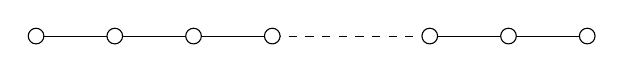
\begin{tikzpicture}
            \draw (0,0) -- (3,0);
            \draw [dashed] (3,0) -- (5,0);
            \draw (5,0) -- (7,0);
            \foreach \x in {0,1,2,3,5,6,7} {
            \node [circle, fill=white, draw=black, inner sep=2pt] at (\x,0) {};
            }
        \end{tikzpicture}
    \end{center}
    图中顶点代表空间 $\left(M(X,\phi_i),z_i+z_i^{-1}\right)$ 与 $P(Y,\xi_i)$，两个顶点之间连一条边，当且仅当它们代表的对象沿纤维/除子粘合。
\end{crl}

\begin{yizhu}[图中的虚线只是「链还没画完」]
实线边表示两块确实沿纤维或除子粘合；虚线边并不表示一种特殊的粘合方式，只表示这条链继续向右延伸、$k$ 可以任意。推论 \ref{crl:gluing-mirror-symmetry-circ} 把首尾两个顶点再连起来之后，链变成环，那条虚线边也就补成了真正的粘合。读这张图时把它当作「粘合示意图」而非几何图形，就不会在虚线上纠缠。
\end{yizhu}

自然，我们还可以把推论 \ref{crl:gluing-mirror-symmetry} 中首尾两个顶点也连起来，从而得到「映射穿孔环面」的镜像对称：

\begin{crl}\label{crl:gluing-mirror-symmetry-circ}
    在与推论 \ref{crl:gluing-mirror-symmetry} 相同的约定下，设 \[
        \mathcal{X}_{\circ} (\phi_1,\dotsb,\phi_k)\quad\text{和}\quad\mathcal{Y}_{\circ} (\xi_1,\dotsb,\xi_k)
    \]分别是按推论 \ref{crl:gluing-mirror-symmetry} 的同一规则、依下图粘合 Weinstein 扇形 $(M(X,\phi_i),z_i+z_i^{-1})$ 与 $\mathbb{P} (\mathcal{O}_Y\oplus\mathcal{L}_{\xi_i})$ 所得的 Weinstein 扇形与代数簇
    \begin{center}
% [原文 p.7]
    \begin{tikzpicture}
        % Circle radius
        \def\R{2}
        % Seven vertices equally spaced around the circle
        \coordinate (v1) at (90:\R);
        \coordinate (v2) at (38.571:\R);
        \coordinate (v3) at (-12.857:\R);
        \coordinate (v4) at (-64.286:\R);
        \coordinate (v5) at (-115.714:\R);
        \coordinate (v6) at (-167.143:\R);
        \coordinate (v7) at (-218.571:\R);
        % Edges, with the fourth-to-fifth edge dashed
        \draw (v1) arc (90:38.571:\R);
        \draw (v2) arc (38.571:-12.857:\R);
        \draw (v3) arc (-12.857:-64.286:\R);
        \draw (v4) arc (-64.286:-115.714:\R);
        \draw[dashed] (v5) arc (-115.714:-167.143:\R);
        \draw (v6) arc (-167.143:-218.571:\R);
        \draw (v7) arc (-218.571:-270:\R);
        % Vertices
        \foreach \vertex in {v1,v2,v3,v4,v5,v6,v7} {
            \node[circle, fill=white, draw=black, inner sep=2pt]
                at (\vertex) {};
        }
    \end{tikzpicture}
\end{center}
    则 $A_{\infty}$-范畴之间存在拟等价 \[
    \Perf\mathcal{W}\left[\mathcal{X}_{\circ} (\phi_1,\dotsb,\phi_k)\right]^{op}\simeq\Coh\mathcal{Y}_{\circ} (\xi_1,\dotsb,\xi_k)_{dg}.
\]
\end{crl}

再配合一些改自 \cite{LK17} 的形变论证，我们应当能实现以椭圆曲线为纤维的纤维丛的镜像对称。

除了把各块粘起来，还可以在 $B$ 侧取线丛的直和，再逐纤维紧化成一个环面丛；相应地，在 $A$ 侧取若干 $T^{\ast}\mathbb{S}^1$ 的乘积，并在底空间上放置相应的停止位，所用规则见 \cite{FLTZ12,Kuwagaki20}。

更精确地说，给定 $A$ 侧的镜像对 $(X;\phi_1,\dotsb ,\phi_k)$ 与 $B$ 侧的镜像对 $(Y;\xi_1,\dotsb, \xi_k)$，其中 $(\phi_1,\dotsb ,\phi_k)$ 是两两交换的辛同胚，再给定整凸多面体 $\Sigma\subseteq\mathbb{R}^k$，可以构造
\[
    \mathcal{X}_{\Sigma} (X;\phi_1,\dotsb ,\phi_k )\coloneqq\left(T^{\ast}\mathbb{T}^n,\Lambda_{\Sigma}\right)\times_{\phi_1,\dotsb ,\phi_n} X\to (T^{\ast}\mathbb{T}^n,\Lambda_{\Sigma})
\]
% [原文 p.8]
作为以 $X$ 为纤维的纤维丛，绕 $\pi_1(\mathbb{T}^n)$ 每个生成元的单值性为 $\phi_i$；同时构造 $\mathcal{Y}_{\Sigma} (Y;\xi_1,\dotsb ,\xi_k)$，它是 $Y$ 上以 $X_{\Sigma}$ 为纤维的纤维丛，$(\xi_1,\dotsb ,\xi_k)$ 刻画其结构主丛。

\begin{yizhu}[原文笔误：$\mathbb{T}^n$ 应为 $\mathbb{T}^k$]
原文这一句前面取的是 $\Sigma\subseteq\mathbb{R}^k$ 与 $\phi_1,\dotsb,\phi_k$，此处却写成 $\mathbb{T}^n$ 与 $\phi_1,\dotsb,\phi_n$；下文又用 $\pi_1(\mathbb{T}^n)$ 的生成元，故按上下文 $n$ 应为 $k$，即环面丛的秩等于多面体 $\Sigma$ 所在空间的维数。译文照原文排印，读到下标 $n$ 时请自行换成 $k$。
\end{yizhu}

\begin{crl}\label{crl:toric-bundle-HMS}
    在与推论 \ref{crl:gluing-mirror-symmetry} 相同的约定下，设 $\Sigma$ 是 $\mathbb{R}^k$ 中的整凸多面体，则 $A_{\infty}$-范畴之间存在拟等价 \[
    \Perf\mathcal{W}\left[\mathcal{X}_{\Sigma} (X;\phi_1,\dotsb ,\phi_k)\right]^{op}\simeq\Coh\left[\mathcal{Y}_{\Sigma} (Y;\xi_1,\dotsb ,\xi_k)\right]_{dg}.
    \]
\end{crl}

\subsection{Hirzebruch 面}

作为另一项应用，我们考察一类特例：作为 $\mathbb{P}^1$ 上 $\mathbb{P}^1$-丛的射影环簇曲面，它们称为 \emph{Hirzebruch 面}。更精确地说，给定非负整数 $n$，Hirzebruch 面 $\mathbb{F}_n$ 是 $\mathbb{P}^1$ 上秩 $2$ 向量丛 $\mathcal{O}\oplus\mathcal{O}_{\mathbb{P}^1} (n)$ 的射影化
\[
    \mathbb{F}_n =\mathbb{P}\left(\mathcal{O}_{\mathbb{P}^1}\oplus\mathcal{O}_{\mathbb{P}^1}(n)\right).
\]
由于 $\mathbb{P}^1$ 是环簇，对一切 $n$，$\mathbb{F}_n$ 都是环簇。

\begin{conceptbox}{Hirzebruch 面}
$\mathbb{F}_n=\mathbb{P}\left(\mathcal{O}_{\mathbb{P}^1}\oplus\mathcal{O}_{\mathbb{P}^1}(n)\right)$ 是 $\mathbb{P}^1$ 上的 $\mathbb{P}^1$-丛；把 $n$ 换成 $-n$ 并交换两个截面即得同构，故同构类型只依赖 $|n|$。$\mathbb{F}_0=\mathbb{P}^1\times\mathbb{P}^1$，而 $\mathbb{F}_1$ 是 $\mathbb{P}^2$ 在一点处的爆破。不同的 $|n|$ 给出互不同构的复结构，但它们作为辛流形可以彼此形变——本文正是借这一点，用同一个映射柱构造在 $\mathbb{F}_n$ 上造出一族「异域」的 Weinstein 扇形（推论 \ref{crl:exotic-Weinstein-structure}）。
\par\smallskip\noindent{\footnotesize 参考：Hartshorne, \emph{Algebraic Geometry}, V.2；本文 §1c。}
\end{conceptbox}

注意，尽管对一切环簇都已知道凝聚—可构造对应，当环簇不是 Fano 时，该结果与 Hori--Vafa \cite{HV00} 的镜像构造并不相容。例如，Hori--Vafa 超势 $W_n$ 的临界点个数不等于镜像 $\mathbb{F}_n$ 的量子上同调秩 \cite[Example 8.2]{FOOO10}。SYZ 镜像构造——如 Auroux \cite{Auroux09} 所解释、后由 Jing \cite{Jing26} 所研究——则高度非平凡，可能涉及把无穷多块图卡粘在一起。

借助定理 \ref{thm:HMS-projective-bundle}，我们给出 $\mathbb{F}_n$ 的同调镜像的一个相当直接的描述。

\begin{crl}\label{crl:mirror-to-Hirzebruch}
    记 \[
        \rF_n =\left(M((\mathbb{C}^{\ast}, x+1/x),\phi^n),z+1/z\right)
    \]为一个 Landau--Ginzburg 模型，其中 $\phi\colon\mathbb{C}^{\ast}=T^{\ast}\mathbb{S}^1\to T^{\ast}\mathbb{S}^1$ 是沿零截面的 Dehn 扭转。则作为带边流形有微分同胚，作为带超势的全纯流形有同构 \[
        \rF_n\cong\left(\mathbb{C}^{\ast}\times\mathbb{C}^{\ast}, x+1/x+y+1/y\right)
    \]并且 $A_{\infty}$-范畴之间存在拟等价 \[
        \Perf\mathcal{W} (\rF_n)^{op}\simeq\Coh\left(\mathbb{F}_n\right)_{dg}.
    \]
\end{crl}

\begin{yizhu}[$\rF_n$ 的记号与「微分同胚不算辛同构」]
$\rF_n$ 中的花体 F 是翻转的 $\mathrm{F}$——它表示 $\mathbb{F}_n$ 的镜像，不是一个新曲面。推论 \ref{crl:mirror-to-Hirzebruch} 同时给出两个层面的结论：作为带边流形微分同胚，作为带超势的全纯流形同构。但微分同胚远弱于精确辛同胚：前者只比对光滑结构，后者要求 Liouville 形式本身被拉回；这里两个结论并不蕴含 $\rF_n$ 与 $\left(\mathbb{C}^{\ast}\right)^2$ 在辛意义下相同，下一推论的「异域」正由此而来。
\end{yizhu}

特别地，由 Bondal--Orlov \cite{BO01} 与 Bridgeland--Maciocia \cite{BM01} 的工作可知，$\Coh (\mathbb{F}_n)\cong\Coh (\mathbb{F}_m)$ 当且仅当 $m=n$，于是立即得到下面这个或许有趣的推论：

\begin{crl}\label{crl:exotic-Weinstein-structure}
    $\rF_n$ 与 $\rF_m$ 精确辛同胚，当且仅当 $m=n$。
\end{crl}

因此，尽管所有 $\rF_n$ 作为 Landau--Ginzburg 对都彼此微分同胚且同构，它们之间却并非精确辛同胚；于是它们构成一族「异域」的 Weinstein 扇形，因为精确辛同胚保持 Fukaya 范畴 \cite{HS26}。不过应当注意，Fukaya 范畴无法区分它们的凸完成，因此我们并不知道这是否在 $\left(\mathbb{C}^{\ast}\right)^2$ 上造出了异域的 Weinstein 结构。另一个疑问是局部同调镜像与 Hori--Vafa 构造之间的关系，即

\begin{conceptbox}{异域 Weinstein 结构}
同一个光滑流形上可以承载无穷多个两两不精确辛同构的 Weinstein 结构：它们作为辛流形彼此不同，其上的包裹 Fukaya 范畴却可能等价。本文由 Hirzebruch 面 $\mathbb{F}_n$（$n\ge 0$）造出这样一族结构——$\rF_n$ 作为带边流形、作为带超势全纯流形都同构，精确辛同构类却随 $n$ 变化，故称「异域」。它说明 A 模型经 $\Coh$ 的等价能看见 B 侧的部分复结构差异，却看不见凸完成层面的差异，这对「Weinstein 结构的辛同胚分类」与「Fukaya 范畴的分类」之间的落差给出了一个具体刻度。
\par\smallskip\noindent{\footnotesize 参考：Kartal, arXiv:2204.04928；本文 §1c 推论 \ref{crl:exotic-Weinstein-structure}。}
\end{conceptbox}

\begin{ques}\label{Q:HV-vs-LHMS}
    局部同调镜像 $\rF_n$ 与 Hori--Vafa 镜像 $\left((\mathbb{C}^{\ast})^2,W_n\right)$ 之间是什么关系？
\end{ques}

回答这个问题有望通过族 Floer 纲领，得到 Hirzebruch 面所期望的 SYZ 镜像。

\begin{keytakeaways}
  \item 多重单值性的机制：把 $k$ 个射影丛 $P(Y,\xi_i)$ 沿零截面与无穷远截面粘成节点链，B 侧的 $\Coh$ 由真下降（同伦前推）拼出；A 侧对应把 $k$ 个映射柱 $(M(X,\phi_i),z_i+z_i^{-1})$ 沿停止位粘成 Weinstein 扇形。推论 \ref{crl:gluing-mirror-symmetry} 与 \ref{crl:gluing-mirror-symmetry-circ} 分别是开链与闭环两种粘法，而推论 \ref{crl:toric-bundle-HMS} 把同一套下降换成环面丛。
  \item 链式粘合的单值性对应很强：B 侧的 $\{P(Y,\xi_i)\}$ 沿截面粘、A 侧的 $\{z_i\}$ 坐标在 $0$ 与 $\infty$ 处相接，$0/\infty$ 的对应关系是全部计算的账本，稍一错位就会得到不同的扇形。
  \item Hirzebruch 面给出显式例子：$\rF_n$ 作为带超势全纯流形，同构于 $\mathbb{C}^{\ast}_x\times\mathbb{C}^{\ast}_y$ 上带超势 $x+1/x+y+1/y$ 的模型，但 $n$ 不同则精确辛同构类不同，根源是 B 侧的 $\Coh (\mathbb{F}_n)$ 不同（推论 \ref{crl:exotic-Weinstein-structure}）。
\end{keytakeaways}

\subsection{全文结构}

在第 \ref{sec:proof-of-theorems} 节中，我们给出主定理各条陈述的全部证明，技术细节留到后面的各节。在第 \ref{sec:algebraic-preparations} 节中，我们给出全文要用到的高阶代数及其相应运算的基本定义。第 \ref{sec:Fukaya-category-discrete-quotient} 节致力于 $A$ 侧计算所需的若干新的结构性结果，第 \ref{sec:G-equiv-sheaves} 节与第 \ref{sec:kunneth-formula} 节则为 $B$ 侧计算准备必要的材料。更具体地说，第 \ref{sec:G-equiv-sheaves} 节给出 $G$-等变层范畴的基本性质，第 \ref{sec:kunneth-formula} 节建立关键公式：等变层的 K\"unneth 公式。在附录 \ref{sec:Eilenberg-Zilber-constraction} 中，我们回顾经典的 Eilenberg--Zilber 构造，并把它改造到本文的情形，它将用于 Künneth 公式 \ref{thm:Kunneth-embedding} 的证明。

% [原文 p.9]
\subsection*{致谢}

本文的主要想法源于 2025 年末作者在波恩马克斯·普朗克数学研究所逗留期间与 Tim Hu、Maximilian Schimpf 的讨论，我们感谢与他们的所有有益讨论。

我们还要感谢 Yanki Lekili、Cheuk Yu Mak、Longke Tang 与 Bingyu Zhang 的许多有益讨论与建议。

S.-Y. Liu 由德国研究基金会（Deutsche Forschungsgemeinschaft，DFG）在德国卓越战略（Germany's Excellence Strategy）项目 GZ 2047/1、Projekt-ID 390685813 下资助。

Kyungmin Rho 感谢波恩马克斯·普朗克数学研究所的款待与资助。

\subsection*{AI 使用声明}

当作者试图证明不同构的 Hirzebruch 面上的凝聚层复形不拟同构时，文献 \cite{BM01} 的结果是在大语言模型（LLM）的帮助下找到的。作者当时认为应当存在比 \cite{BM01} 这一过强结果更合适的参考文献，而 LLM 坚称该结果不可或缺。

作者用 LLM 探究 \ref{defn:wrapped-Fukaya-cat-inf-sectors} 中「小」Fukaya 范畴的定义是否就是 $\mathcal{W}^{big} (X)$ 中紧对象的范畴，未能成功。在与 Bingyu Zhang、Longke Tang 讨论之后，作者确信需要一些必要的几何论证，于是决定把这一点留作后续问题。

把 $A_{\infty}$-范畴 $\mathcal{A}$ 关于群 $G$ 的同伦商与 $A_{\infty}$-轨道范畴联系起来的文献 \cite{Christ26}，同样是在 LLM 的帮助下找到的。

在推论 \ref{crl:gluing-mirror-symmetry} 的证明中，作者请 LLM 把第一个巨大的公式拆成两行：原始代码输入 LLM，输出经检查后直接复制进文件。

作者曾尝试为命题 \ref{prp:dg-enhancement} 的证明寻找更多参考文献，LLM 未能给出超出作者已有知识范围的答案。

作者用 LLM 把 Seidel \cite{Seidel08} 的右模作用改写为左模作用，检查后把生成的代码复制进文件。
